\begin{figure*}
  \centering
  \begin{subfigure}[b]{\textwidth}
    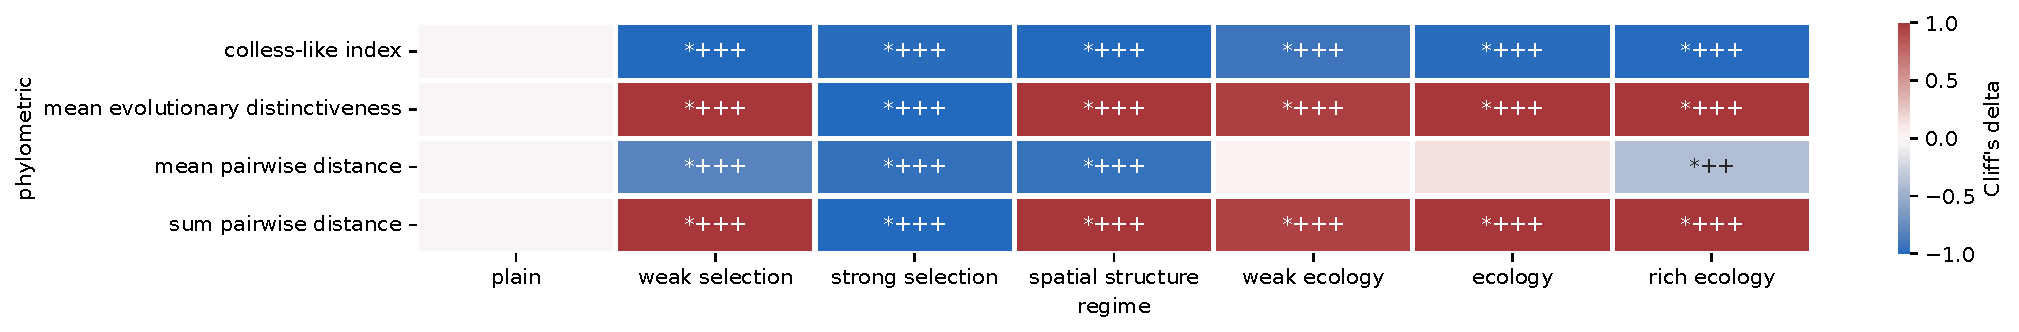
\includegraphics[width=\textwidth]{binder/binder/teeplots/epoch=7+mut_distn=np.random.standard_normal+viz=heatmap+x=regime+y=phylometric+ext=.pdf}
    \caption{Reference phylogeny.}
  \end{subfigure}%
\begin{subfigure}[b]{\textwidth}
  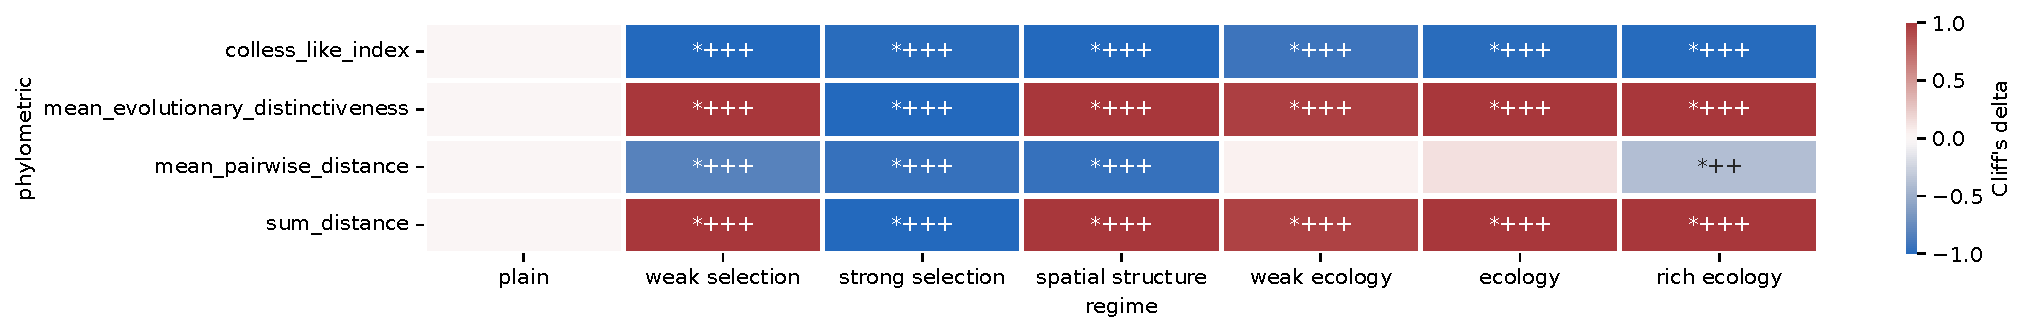
\includegraphics[width=\textwidth]{binder/binder/teeplots/epoch=7+mut_distn=np.random.standard_normal+resolution=100.0+viz=heatmap+x=regime+y=phylometric+ext=.pdf}
  \caption{1\% resolution reconstruction.}
\end{subfigure}%
\begin{subfigure}[b]{\textwidth}
  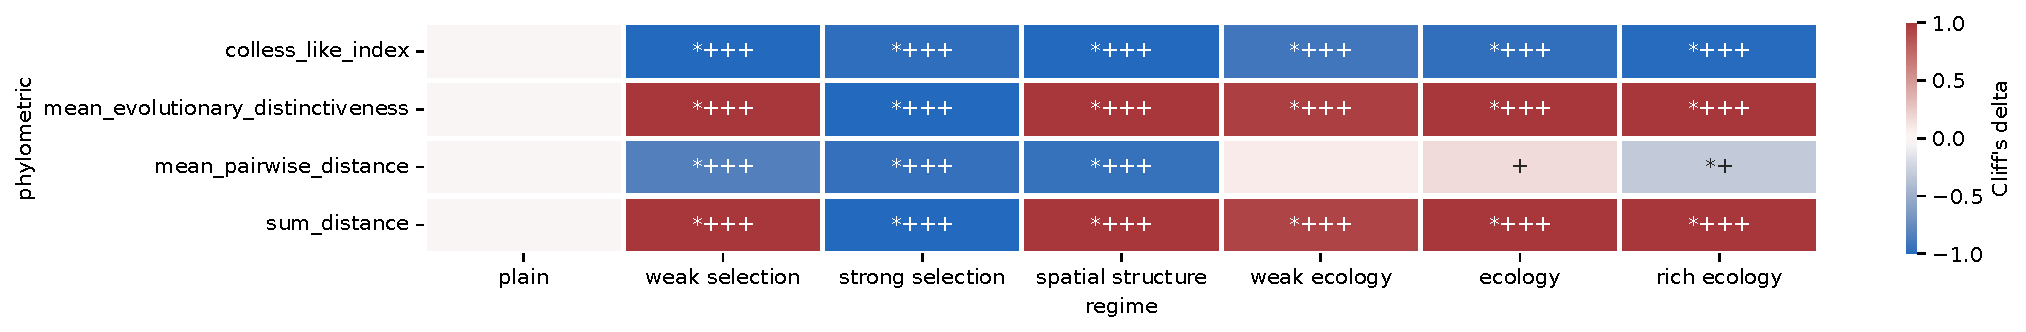
\includegraphics[width=\textwidth]{binder/binder/teeplots/epoch=7+mut_distn=np.random.standard_normal+resolution=30.0+viz=heatmap+x=regime+y=phylometric+ext=.pdf}
  \caption{3\% resolution reconstruction.}
\end{subfigure}%
\begin{subfigure}[b]{\textwidth}
  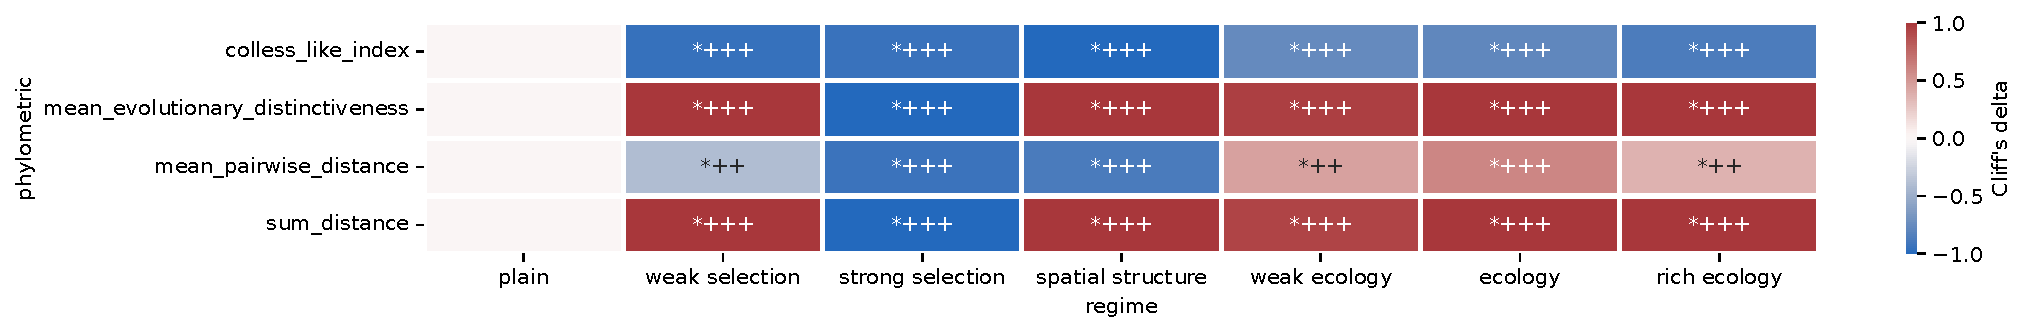
\includegraphics[width=\textwidth]{binder/binder/teeplots/epoch=7+mut_distn=np.random.standard_normal+resolution=10.0+viz=heatmap+x=regime+y=phylometric+ext=.pdf}
  \caption{10\% resolution reconstruction.}
\end{subfigure}%
\begin{subfigure}[b]{\textwidth}
  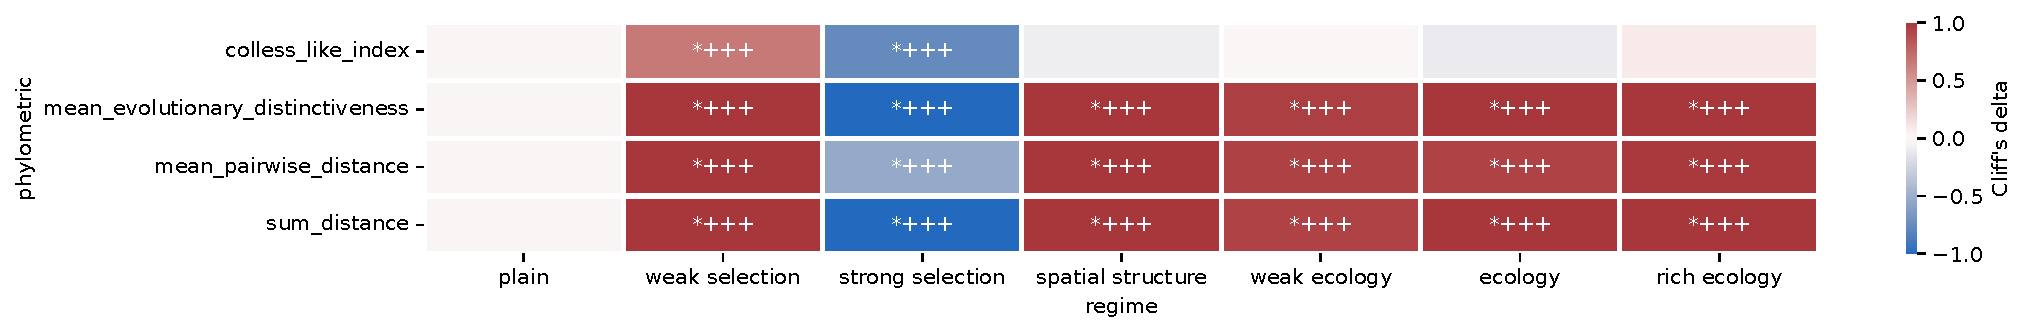
\includegraphics[width=\textwidth]{binder/binder/teeplots/epoch=7+mut_distn=np.random.standard_normal+resolution=3.0+viz=heatmap+x=regime+y=phylometric+ext=.pdf}
  \caption{30\% resolution reconstruction.}
\end{subfigure}%
  \caption{
Tree phylometrics across surveyed evolutionary regimes, calculated on reconstructed and perfect-fidelity simulation phylogenetic records from simple model.
Note that nonparametric effect size normalization caps out to 1.0/-1.0 past the point of complete disbributional nonoverlap.
For heatmap charts, +'s indicate small, medium, and large effect sizes using the Cliff's delta statistic and *'s indicate statistical significance at $\alpha = 0.05$ via Mann-Whitney U test.
Results from simple model are for standard experimental conditions: gaussian mutation distribution at epoch 7 (generation 262,144).
  }
  \label{fig:reconstructed-tree-phylometrics-progressive-heatmap}
\end{figure*}